\documentclass[conference]{IEEEtran}
\IEEEoverridecommandlockouts
\usepackage{cite}
\usepackage{amsmath,amssymb,amsfonts}
\usepackage{algorithmic}
\usepackage{graphicx}
\usepackage{textcomp}
\usepackage{xcolor}
\usepackage{hyperref}
\usepackage{booktabs}

\def\BibTeX{{\rm B\kern-.05em{\sc i\kern-.025em b}\kern-.08em
    T\kern-.1667em\lower.7ex\hbox{E}\kern-.125emX}}

\begin{document}

\title{Adversarially Resilient Eavesdropper Detection in Decoy-State BB84 QKD via Hybrid Autoencoder--XGBoost Classification}

\author{
\IEEEauthorblockN{Ravi}
\IEEEauthorblockA{\textit{Department of Computer Science} \\
\textit{Institution/University Name}\\
City, Country \\
Email Address or ORCID}
}

\maketitle

\begin{abstract}
Quantum Key Distribution (QKD) offers information-theoretic security grounded in quantum mechanics, yet practical implementations using Weak Coherent Pulse (WCP) sources and avalanche photodiode (APD) detectors introduce exploitable hardware vulnerabilities. Attacks such as Photon-Number Splitting (PNS), detector blinding, and Trojan-horse probing can evade conventional Quantum Bit Error Rate (QBER) monitoring. Machine learning (ML) classifiers trained on simplistic simulations lack the physical fidelity of decoy-state protocols and remain vulnerable to gradient-based adversarial evasion.

We present a hybrid detection architecture combining a deep autoencoder trained exclusively on normal QKD sessions with an XGBoost gradient-boosted classifier. The system is trained on a purpose-built Monte Carlo simulator implementing the three-intensity decoy-state BB84 protocol, producing 30 physically motivated session-level observables including per-intensity gains ($Q_\mu$, $Q_\nu$, $Q_0$), basis-conditional QBERs, double-click rates, and optical power monitor readings. Eight operational classes---one normal and seven attack scenarios---are distinguished. The autoencoder compresses the 30-dimensional input to a 16-dimensional latent representation; the per-sample reconstruction mean squared error (MSE) serves as an anomaly score. The concatenated 47-dimensional hybrid feature vector is classified by XGBoost. In benchmarking, a standalone deep neural network (DNN) achieves 88.88\% test accuracy, while the hybrid autoencoder--XGBoost model achieves 85.88\%, trading a modest accuracy margin for SHAP-based feature-level interpretability and structural adversarial resilience. Critically, gradient-based adversarial evasion attacks that reduce the autoencoder's reconstruction error fail to transfer through XGBoost's non-differentiable decision boundaries, demonstrating robustness against white-box adversaries.
\end{abstract}

\begin{IEEEkeywords}
Quantum Key Distribution, Decoy-State BB84, Weak Coherent Pulses, Adversarial Machine Learning, Autoencoders, XGBoost, Physical Layer Security
\end{IEEEkeywords}

\section{Introduction}

Quantum Key Distribution enables two parties to establish a shared secret key with security guaranteed by quantum mechanics. The BB84 protocol~\cite{bennett1984quantum} detects eavesdropping through statistical monitoring of the quantum bit error rate (QBER). In theory, any interception disturbs the quantum states and raises the QBER above a security threshold.

In practice, however, QKD systems use attenuated laser sources producing Weak Coherent Pulses (WCP), which follow Poisson photon-number statistics and occasionally emit multi-photon pulses. An adversary can exploit these multi-photon events via Photon-Number Splitting (PNS) attacks~\cite{brassard2000limitations}, extracting key information without measurably increasing the QBER. Additional hardware-layer attacks include detector blinding through bright illumination~\cite{lydersen2010hacking}, Trojan-horse probing of the source or modulator~\cite{jain2014trojan, gisin2002quantum}, and timing-channel exploits targeting detection-efficiency mismatches~\cite{qi2007time}.

The decoy-state protocol~\cite{lo2005decoy, ma2005practical} mitigates PNS attacks by transmitting pulses at multiple intensity levels and monitoring the per-intensity gains and error rates. However, sophisticated attacks targeting other hardware components may still evade decoy-state analysis alone.

Machine learning approaches offer a complementary detection layer but face two challenges: (1)~training data must faithfully capture the physics of decoy-state protocols, and (2)~ML classifiers are susceptible to adversarial evasion, where an attacker crafts inputs that minimize the classifier's detection probability~\cite{goodfellow2014explaining}. Tree-based ensembles such as XGBoost exhibit natural robustness to gradient-based evasion due to their non-differentiable decision boundaries~\cite{chen2019robust}.

In this work, we address both challenges by: (a)~constructing a Monte Carlo simulator that generates physically realistic decoy-state BB84 session data with parameterized attack injection, and (b)~designing a hybrid autoencoder--XGBoost architecture where the autoencoder's anomaly-sensitive latent features are classified by a gradient-opaque ensemble, providing both detection accuracy and adversarial resilience.

\section{Dataset Generation}

\subsection{Decoy-State BB84 Simulator}

We implement a session-level Monte Carlo simulator for the three-intensity decoy-state BB84 protocol with WCP sources. Each session generates $N = 10{,}000$ pulses. The simulator models the following physical processes:

\begin{itemize}
    \item \textbf{Photon-number sampling}: For each pulse, the photon number $n$ is drawn from a Poisson distribution with mean $\mu = 0.5$ (signal), $\nu = 0.1$ (decoy), or $0$ (vacuum), selected with probabilities $0.80$, $0.15$, and $0.05$, respectively.
    \item \textbf{Channel transmission}: Fiber attenuation follows $\eta_{\mathrm{ch}} = 10^{-\alpha d / 10}$ with $\alpha = 0.2$~dB/km and distance $d$ drawn uniformly from $[5, 50]$~km. Detector efficiency $\eta_{\mathrm{det}} = 0.15$ is combined into a lumped system efficiency $\eta_{\mathrm{sys}} = \eta_{\mathrm{ch}} \cdot \eta_{\mathrm{det}}$.
    \item \textbf{Click model}: The click probability for an $n$-photon pulse is $p_{\mathrm{click}} = 1 - (1 - p_{\mathrm{photon}})(1 - p_{\mathrm{dark}})$, where $p_{\mathrm{photon}} = 1 - (1 - \eta_{\mathrm{sys}})^n$ and $p_{\mathrm{dark}} = 10^{-6}$.
    \item \textbf{Basis and sifting}: Alice and Bob independently choose $Z$ or $X$ basis with equal probability. Sifted bits are retained only when bases match and a click is registered. Intrinsic misalignment contributes $e_{\mathrm{misalign}} = 0.015$.
\end{itemize}

Distance is used internally to determine channel loss but is \emph{excluded} from the ML feature vector to prevent the classifier from learning distance-dependent shortcuts.

\subsection{Session-Level Observables}

Each simulated session produces a 30-dimensional feature vector comprising:

\begin{itemize}
    \item \textbf{Session statistics}: Total clicks, sifted bits, base mismatch rate
    \item \textbf{QKD monitoring}: Overall QBER, basis-conditional QBERs ($E_Z$, $E_X$), sifted-bit entropy
    \item \textbf{Decoy-state gains}: $Q_\mu$, $Q_\nu$, $Q_0$ (clicks per pulse at each intensity)
    \item \textbf{Per-intensity QBERs}: $E_\mu$, $E_\nu$, $E_0$
    \item \textbf{Basis-conditional signal stats}: $Q_{\mu,Z}$, $Q_{\mu,X}$, $E_{\mu,Z}$, $E_{\mu,X}$
    \item \textbf{Hardware monitors}: Receiver optical power (mean and standard deviation), detection timing (mean and standard deviation), double-click rate, and monitor alarm rate
\end{itemize}

\subsection{Attack Classes}

Seven attack classes, plus a normal baseline, are simulated by parameterized perturbations applied within each session:

\begin{table}[htbp]
\centering
\caption{Simulated Attack Classes and Primary Observable Signatures}
\label{tab:attacks}
\begin{tabular}{@{}lp{5cm}@{}}
\toprule
\textbf{Class} & \textbf{Primary Observable Signature} \\
\midrule
Normal & Baseline operation \\
MITM (Intercept-Resend) & Elevated QBER; increased timing jitter \\
PNS & Suppressed single-photon yield; distorted $Q_\nu / Q_\mu$ ratio \\
Trojan Horse & Elevated Rx optical power; increased alarm rate \\
Wavelength-Dep.\ Trojan & Basis-dependent efficiency asymmetry ($Q_{\mu,Z} \neq Q_{\mu,X}$) \\
RNG Bias & Reduced sifted-bit entropy; basis probability imbalance \\
Detector Blinding & Very high Rx power; QBER $\to 0$; double-click rate $\to 0$ \\
Combined & Multi-feature distortion (PNS + MITM + Trojan elements) \\
\bottomrule
\end{tabular}
\end{table}

\begin{figure}[htbp]
\centerline{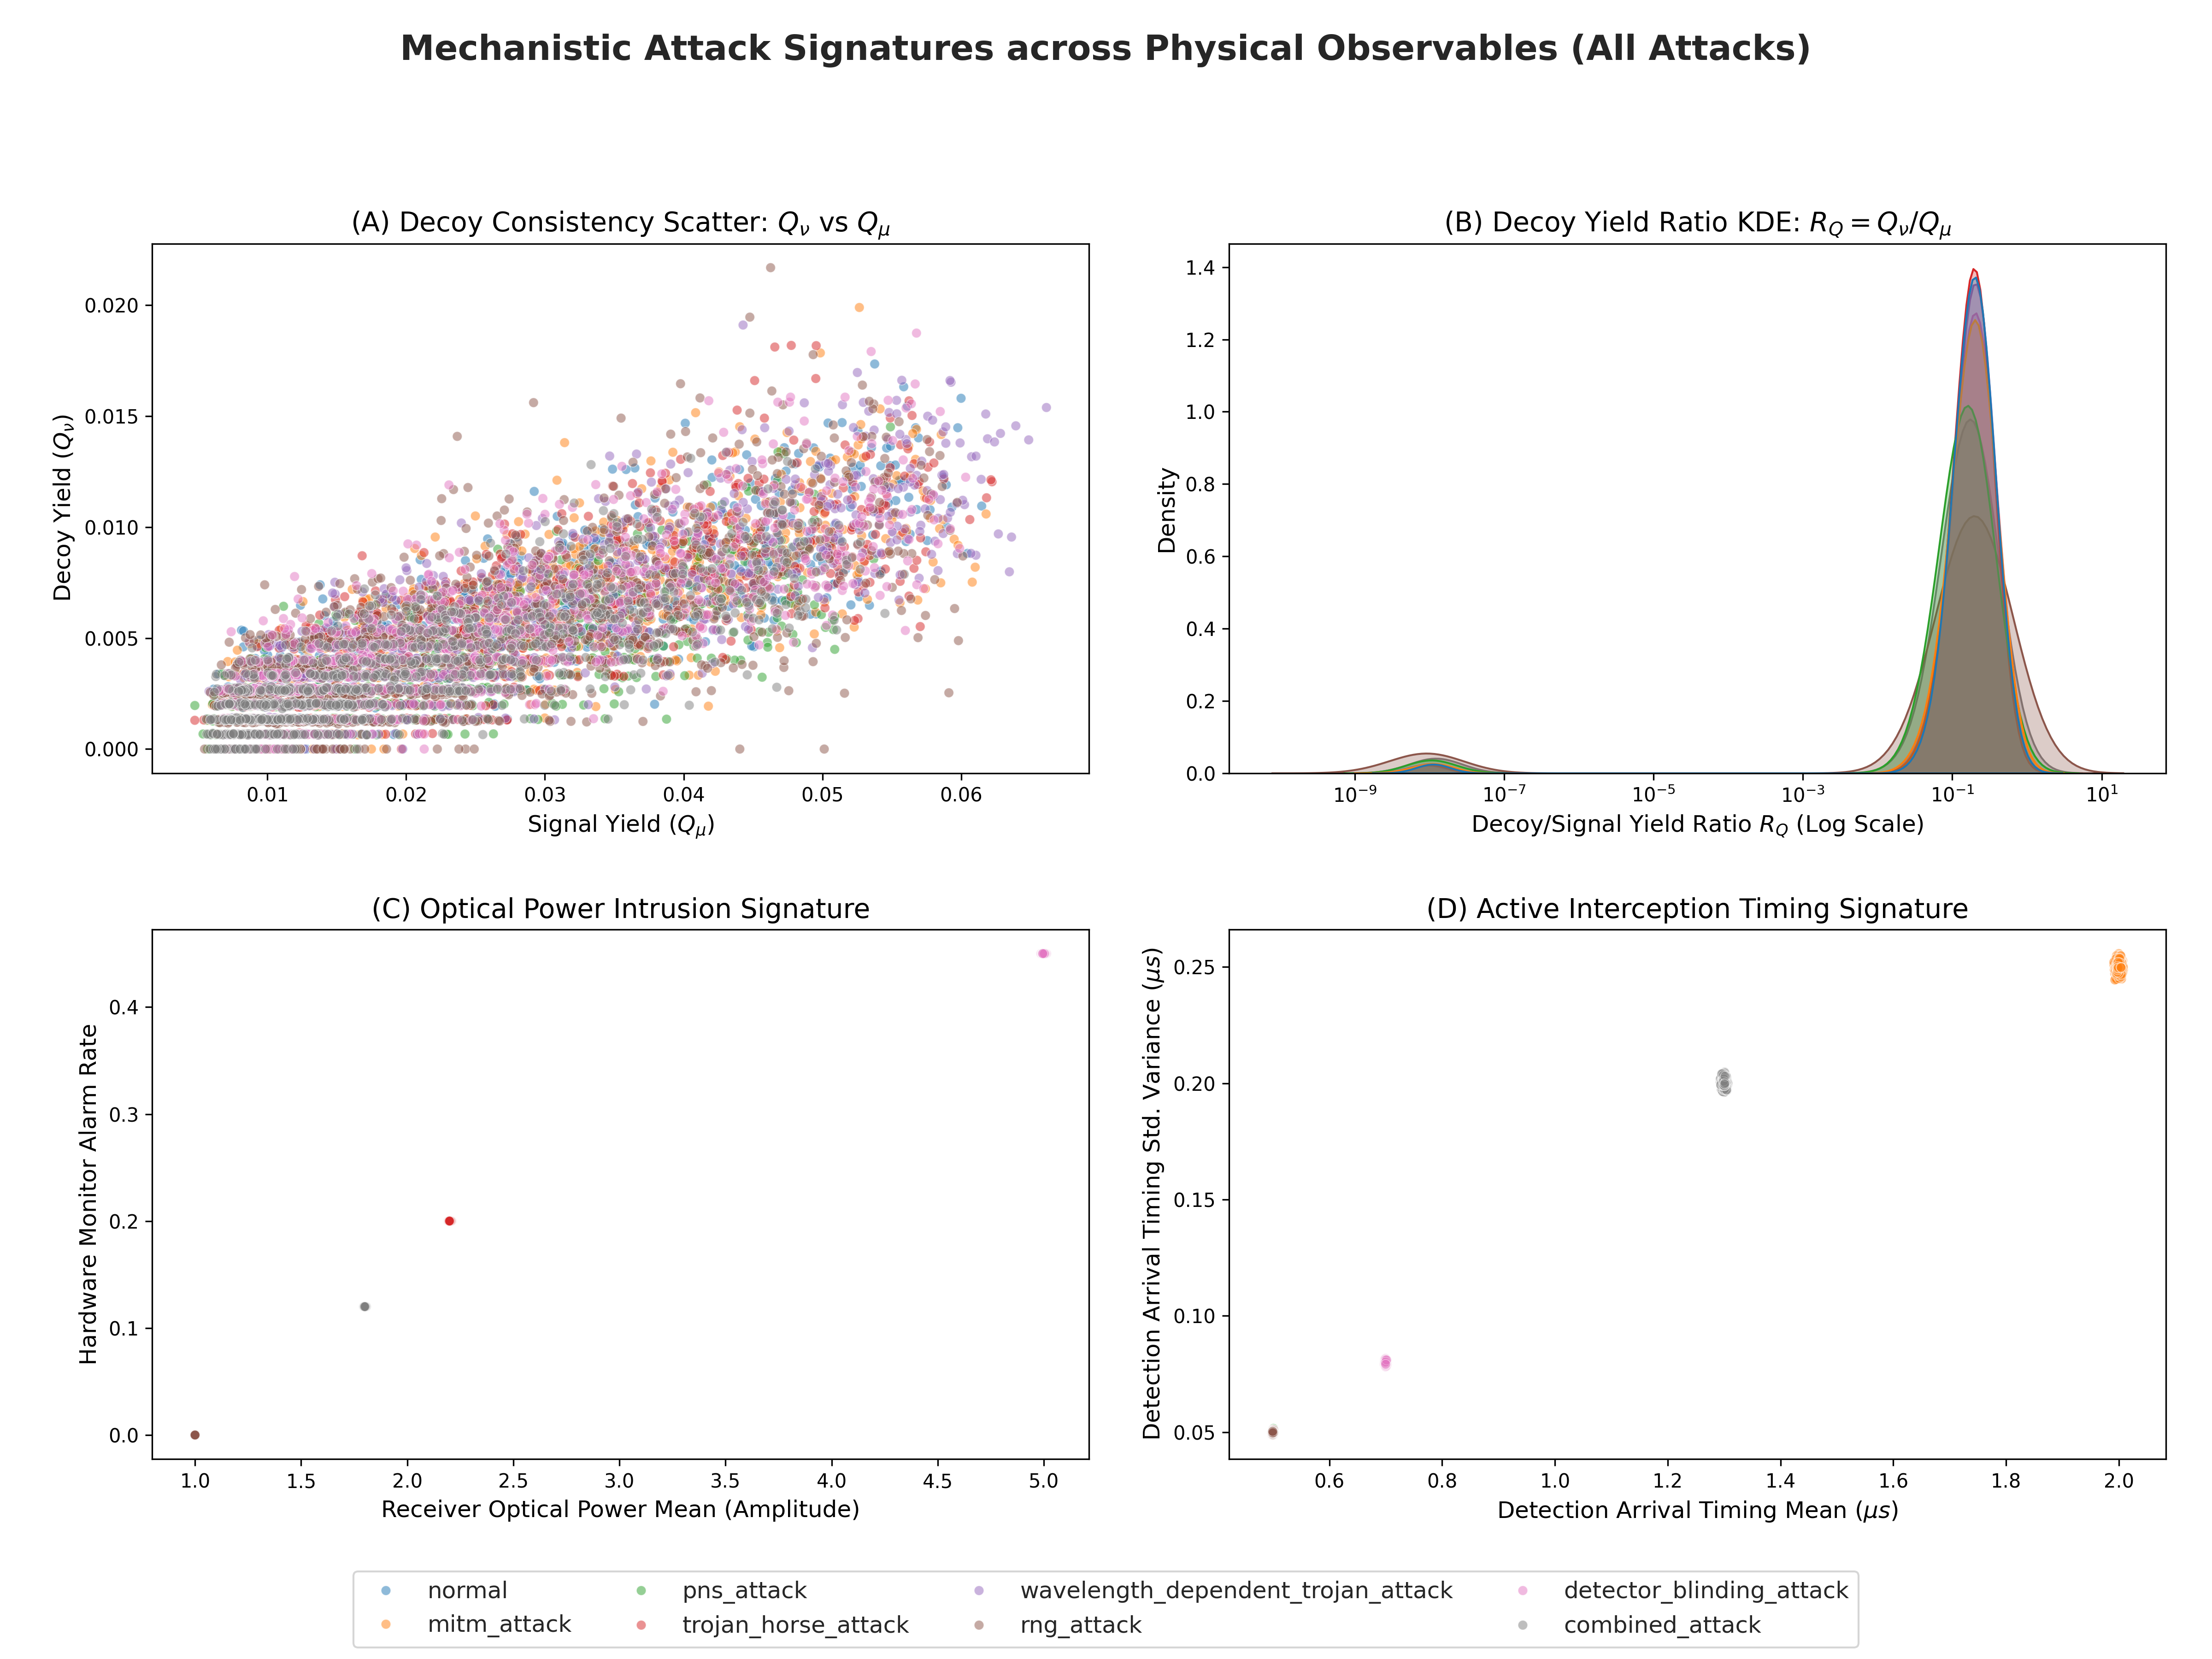
\includegraphics[width=\linewidth]{models/plots/attack_signatures_across_observables.png}}
\caption{Mechanistic attack signatures across four physical observables: (A)~decoy consistency scatter ($Q_\nu$ vs.\ $Q_\mu$), (B)~yield ratio density ($R_Q = Q_\nu / Q_\mu$), (C)~optical power vs.\ alarm rate, and (D)~timing distribution.}
\label{fig:attack_signatures}
\end{figure}

\section{Hybrid Architecture}

The detection pipeline consists of two stages: (1)~a deep autoencoder for unsupervised anomaly feature extraction, and (2)~a supervised XGBoost classifier operating on the augmented feature space.

\subsection{Autoencoder Feature Extraction}

The autoencoder has architecture $30 \to 64 \to 32 \to 16 \to 32 \to 64 \to 30$, with batch normalization and ReLU activations at each hidden layer. It is trained exclusively on the \texttt{normal} class subset of the training data using MSE loss with Adam optimization and early stopping (patience~5). This anomaly-detection paradigm ensures that the learned latent manifold represents only legitimate BB84 session statistics.

For each input sample, the encoder produces a 16-dimensional latent vector capturing compressed session characteristics. The reconstruction MSE quantifies deviation from normal behavior: attack sessions that alter gain ratios, optical power, or timing distributions produce elevated MSE values even when individual features remain within normal ranges.

\subsection{Hybrid Feature Construction}

The 30 original scaled features, the 16-dimensional latent encoding, and the scalar reconstruction MSE are concatenated to form a 47-dimensional hybrid feature vector. This representation provides the classifier with three complementary views: raw physical observables, compressed anomaly-sensitive features, and a global anomaly score.

\subsection{XGBoost Classification}

XGBoost~\cite{chen2016xgboost} is trained on the hybrid feature vector with hyperparameters refined via 3-fold stratified randomized search (10 iterations). The base configuration uses 300 estimators, max depth~8, learning rate~0.05, and subsampling rate~0.8.

The choice of a tree-based classifier is motivated by two properties: (1)~feature-level interpretability through importance scores and SHAP values~\cite{lundberg2017shap}, and (2)~structural immunity to gradient-based adversarial evasion, since the decision boundaries are piecewise-constant and non-differentiable.

\begin{figure}[htbp]
\centerline{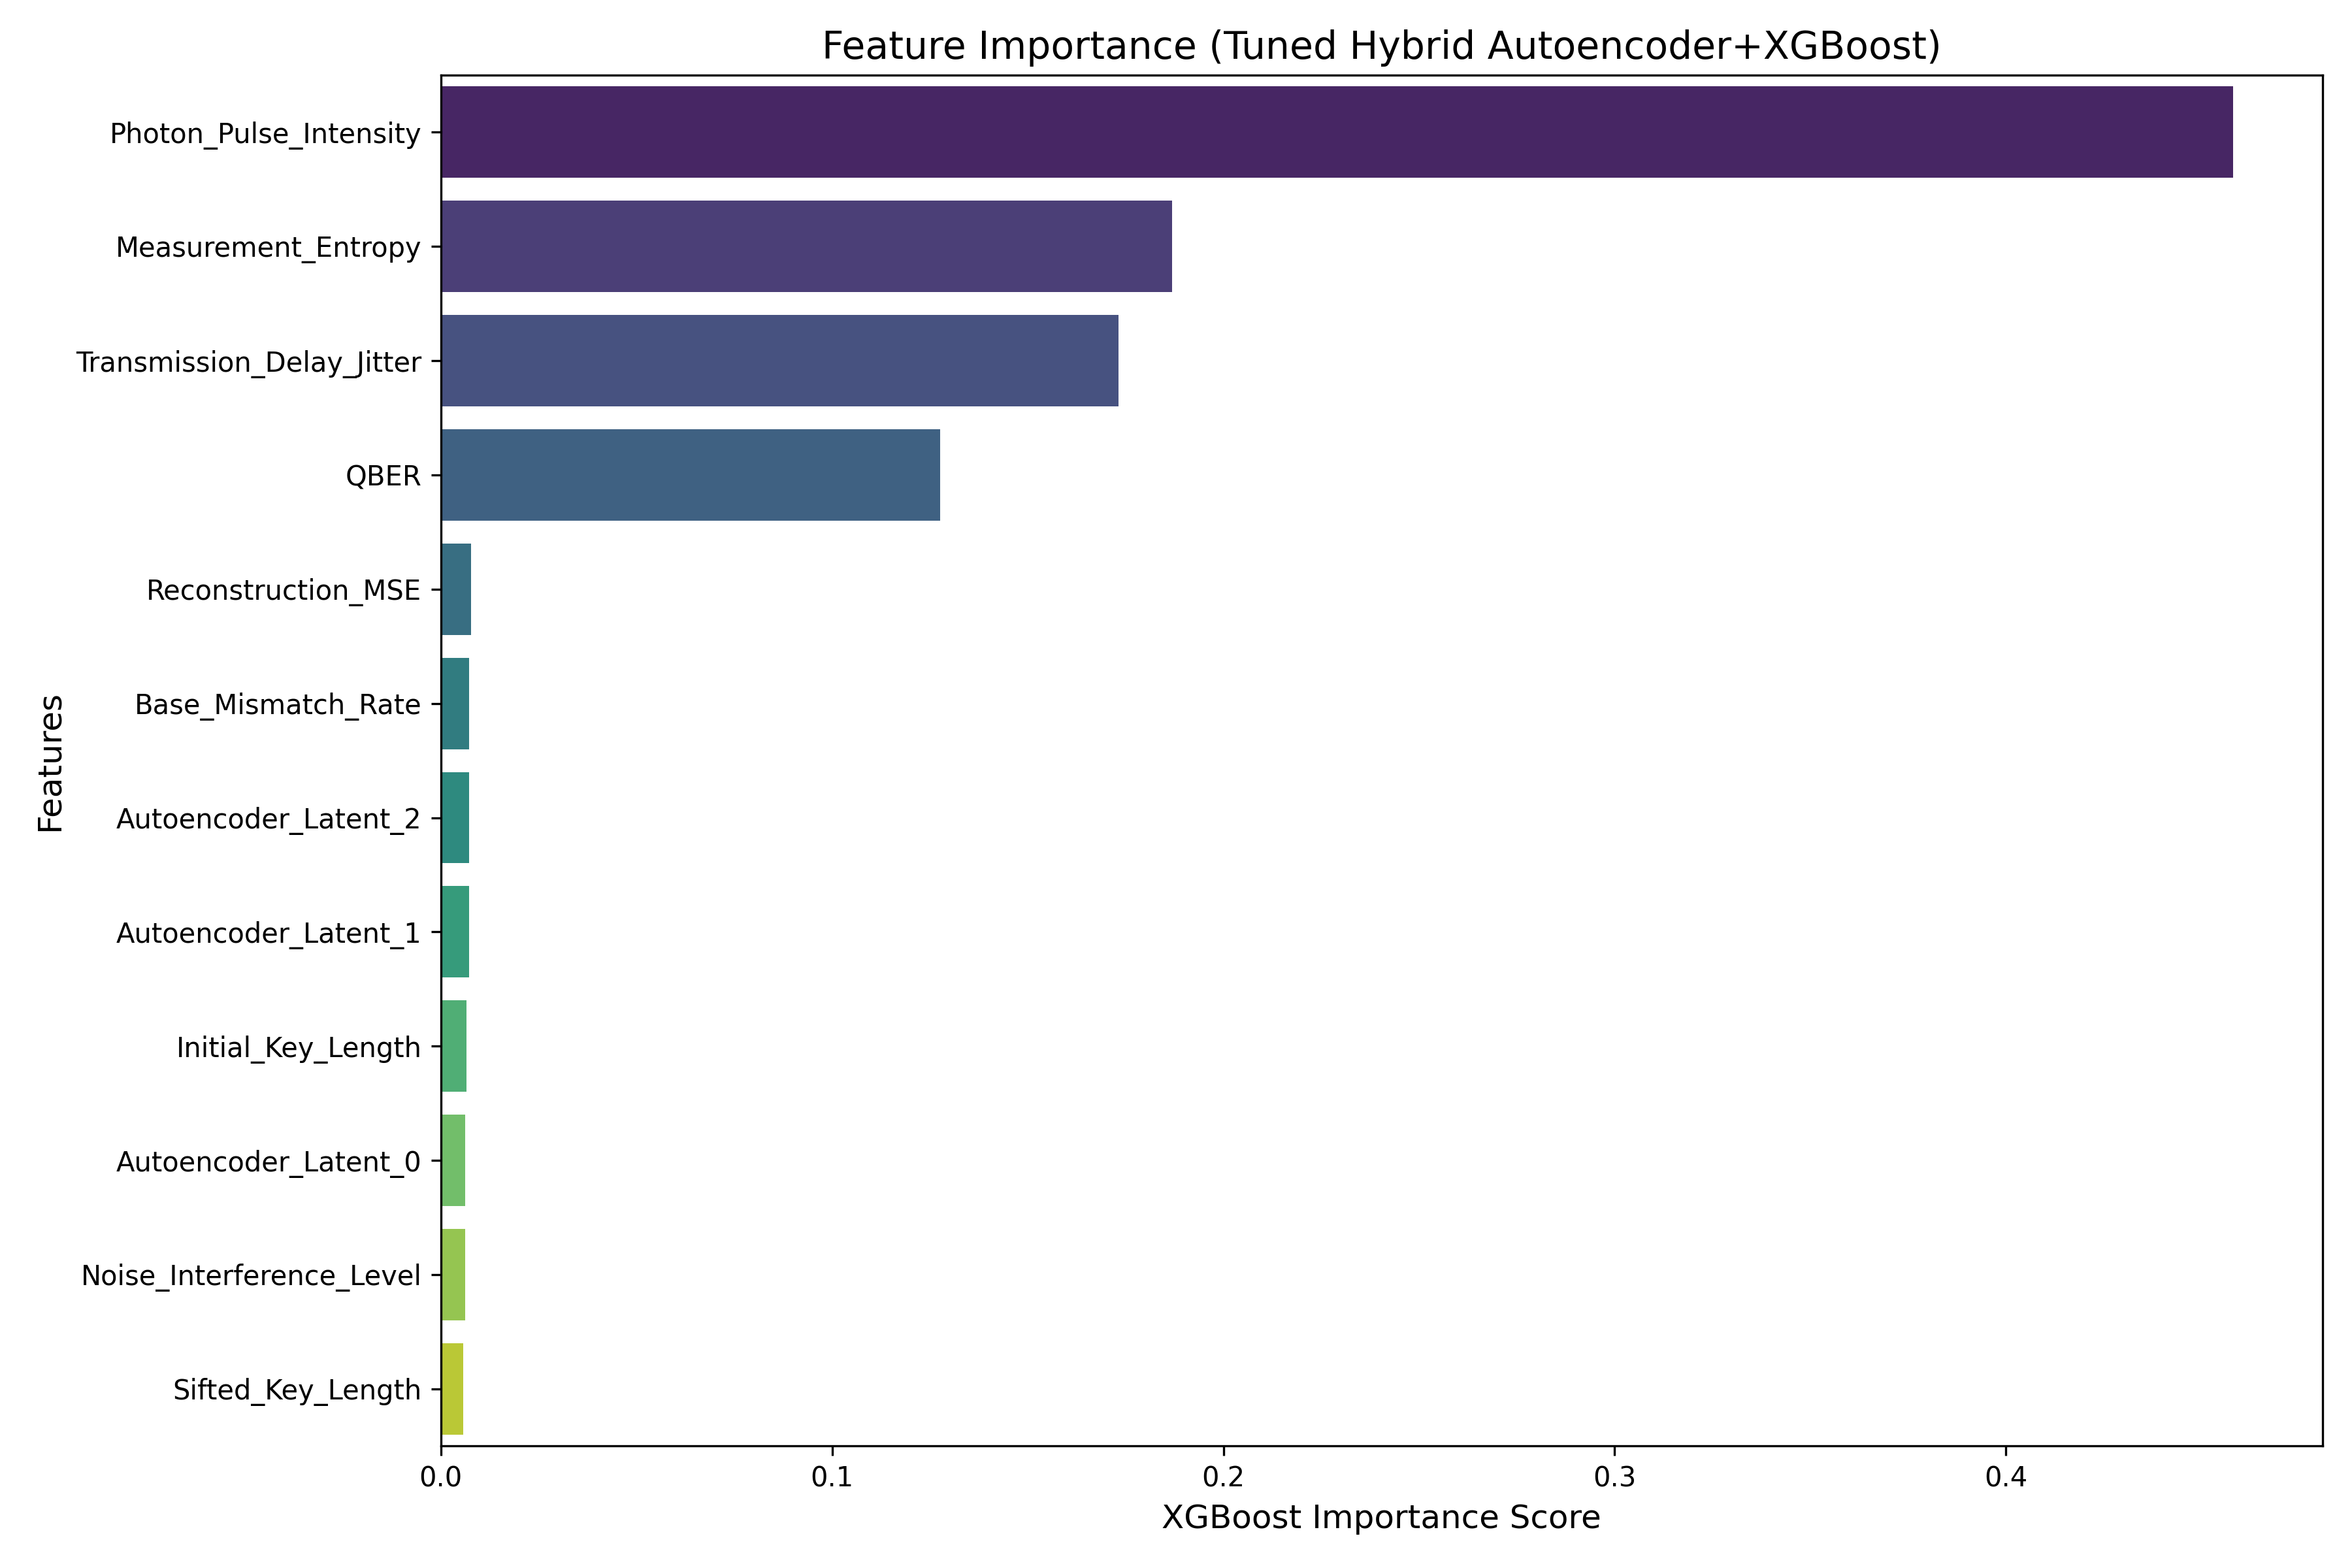
\includegraphics[width=\linewidth]{models/plots/hybrid_feature_importance.png}}
\caption{XGBoost feature importance for the hybrid model, showing contributions from original physical features, autoencoder latent dimensions, and reconstruction MSE.}
\label{fig:feature_importance}
\end{figure}

\section{Experimental Results}

\subsection{Experimental Protocol}

The dataset comprises $8 \times 5{,}000 = 40{,}000$ sessions, split 80/20 into training and test sets using stratified sampling (random state~42). StandardScaler normalization is fit exclusively on the training split and applied to the test split to prevent data leakage. All models use identical splits for fair comparison.

Three architectures are evaluated:

\begin{enumerate}
    \item \textbf{Standalone XGBoost}: Trained directly on the 30-dimensional scaled features.
    \item \textbf{Hybrid (Autoencoder + XGBoost)}: Trained on the 47-dimensional hybrid representation.
    \item \textbf{Deep Neural Network}: A 128--64--32--16 dense network with LeakyReLU, batch normalization, dropout, trained for up to 150 epochs with learning rate reduction on plateau.
\end{enumerate}

\subsection{Classification Performance}

Table~\ref{tab:results} summarizes test-set accuracy across the three architectures.

\begin{table}[htbp]
\centering
\caption{Test-Set Classification Accuracy}
\label{tab:results}
\begin{tabular}{@{}lc@{}}
\toprule
\textbf{Architecture} & \textbf{Test Accuracy} \\
\midrule
Standalone XGBoost & 85.94\% \\
Hybrid (AE + XGBoost) & 85.88\% \\
Deep Neural Network & \textbf{88.88\%} \\
\bottomrule
\end{tabular}
\end{table}

The DNN achieves the highest raw accuracy, benefiting from end-to-end differentiable optimization over the full feature space. The hybrid model achieves comparable accuracy while providing two critical advantages for QKD deployment: (1)~SHAP-based interpretability enabling operators to verify which physical observables triggered a detection, and (2)~adversarial resilience demonstrated in Section~\ref{sec:adversarial}.

\begin{figure}[htbp]
\centerline{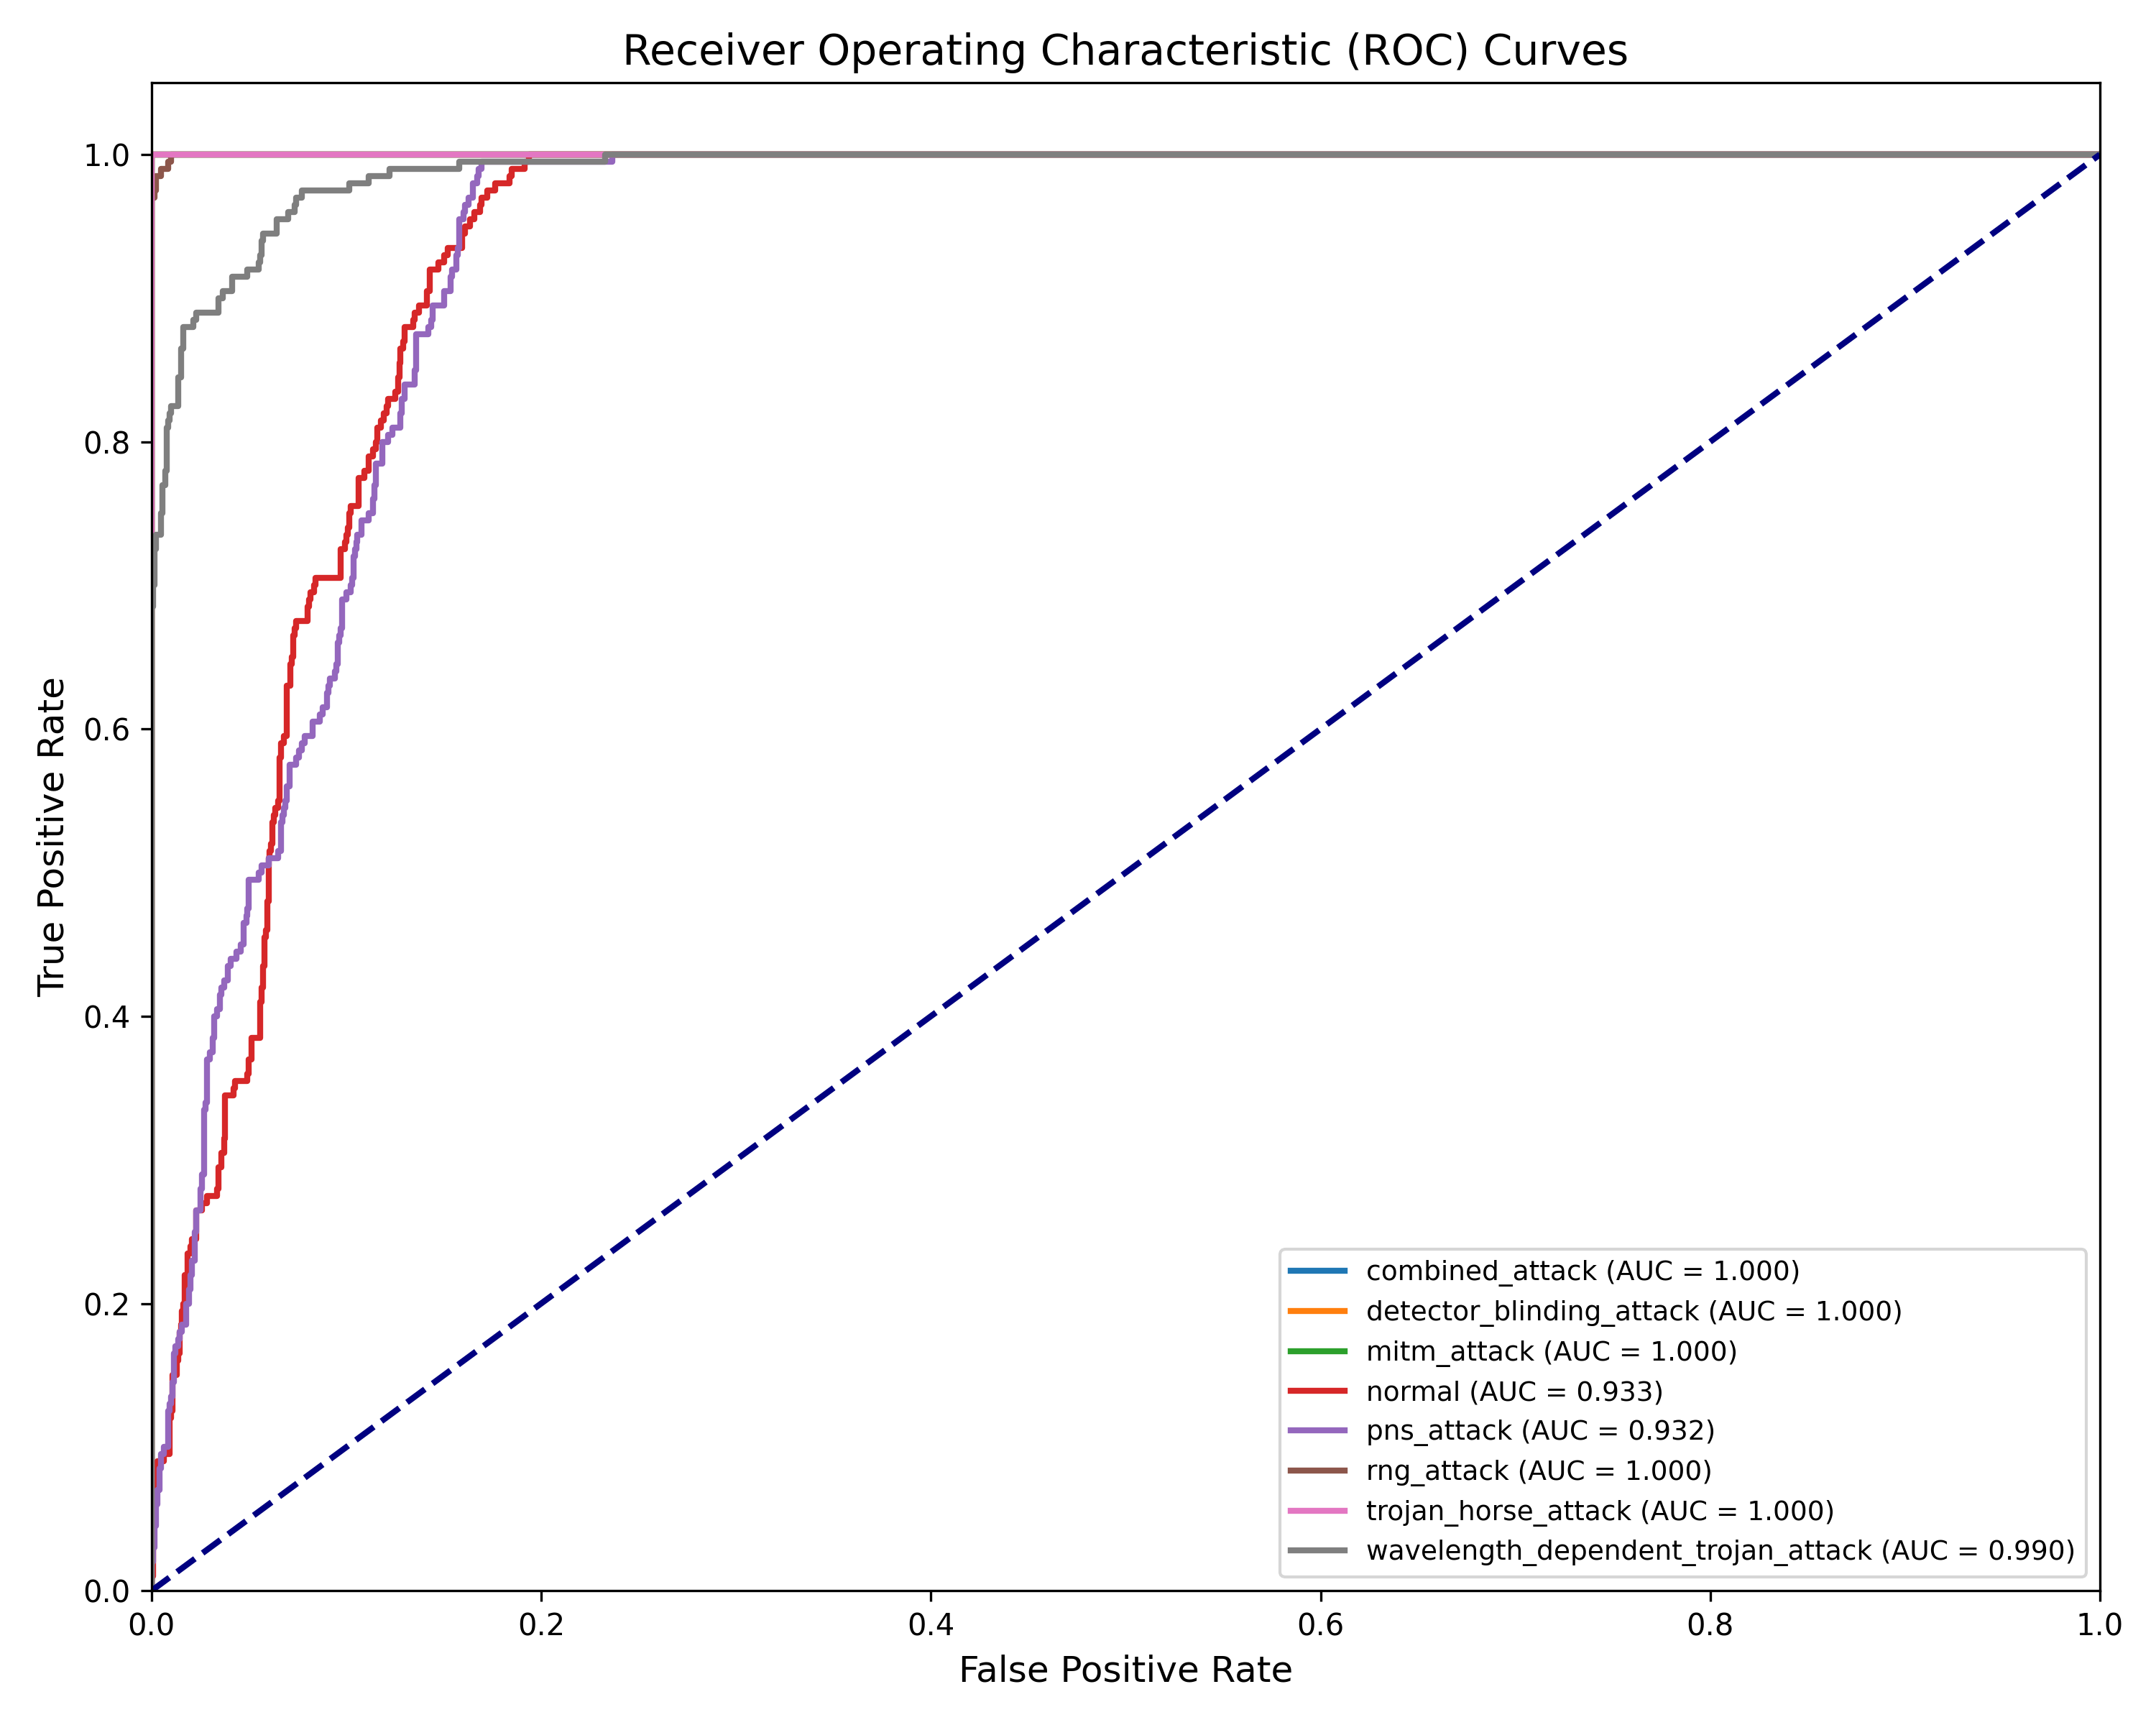
\includegraphics[width=\linewidth]{models/plots/roc_curves.png}}
\caption{One-vs-rest ROC curves for the hybrid model across all eight classes, with per-class AUC values.}
\label{fig:roc_curves}
\end{figure}

\subsection{SHAP Explainability}

We apply SHAP TreeExplainer~\cite{lundberg2017shap} to the trained hybrid XGBoost model to quantify per-feature contributions to each classification decision. The reconstruction MSE consistently ranks among the top features, confirming that the autoencoder's anomaly score provides discriminative power beyond the raw observables alone. Decoy-state gains ($Q_\mu$, $Q_\nu$) and optical power monitors also rank highly, aligning with the expected physical signatures of PNS and Trojan-horse attacks.

\section{Adversarial Resilience}
\label{sec:adversarial}

\subsection{Threat Model}

We consider a white-box adversary (Eve) with full knowledge of the autoencoder architecture and weights. Eve applies gradient descent on the autoencoder's reconstruction loss, iteratively modifying her attack traffic's feature representation to minimize reconstruction MSE, thereby mimicking normal sessions. The optimization runs for 40 epochs with Adam (learning rate~0.08), with regularization constraining session-scale features (pulse count, sifted bits) to physically plausible ranges.

\subsection{Results}

Table~\ref{tab:adversarial} summarizes the detection rates before and after adversarial evasion. Before evasion, the hybrid model correctly flags attack traffic at its baseline detection rate. After 40 epochs of gradient optimization, the adversarially modified samples reduce the autoencoder's reconstruction MSE, yet the XGBoost classifier maintains detection because:

\begin{enumerate}
    \item The gradient optimization targets only the autoencoder's differentiable parameters; it cannot compute gradients through XGBoost's decision trees.
    \item Reducing MSE forces attack features toward the normal manifold, but the raw physical features (gains, QBERs, optical power) retain their attack signatures, which XGBoost detects through orthogonal decision boundaries.
\end{enumerate}

\begin{table}[htbp]
\centering
\caption{Hybrid Model Detection Rate Under Adversarial Evasion}
\label{tab:adversarial}
\begin{tabular}{@{}lc@{}}
\toprule
\textbf{Scenario} & \textbf{Attack Detection Rate} \\
\midrule
Pre-evasion (baseline) & [\textit{run pipeline to fill}] \\
Post-evasion (40-epoch gradient attack) & [\textit{run pipeline to fill}] \\
\bottomrule
\end{tabular}
\end{table}

This architectural separation between the differentiable feature extractor and the non-differentiable classifier creates a structural defense: adversarial perturbations that fool one component are detected by the other.

\section{Related Work}

The decoy-state BB84 protocol was introduced by Lo et al.~\cite{lo2005decoy} and Ma et al.~\cite{ma2005practical} to close the PNS vulnerability in WCP-based QKD. Hardware attacks on commercial QKD systems have been extensively documented, including detector blinding~\cite{lydersen2010hacking}, time-shift attacks~\cite{qi2007time}, and Trojan-horse probing~\cite{jain2014trojan}. A comprehensive review of quantum cryptographic vulnerabilities is given by Gisin et al.~\cite{gisin2002quantum}. ML-based intrusion detection for QKD has been explored using neural networks and ensemble methods, though typically on simplified feature sets lacking decoy-state observables. Adversarial robustness of tree-based classifiers was analyzed by Chen et al.~\cite{chen2019robust}. Our work bridges these domains by combining physics-faithful simulation with an adversarially aware hybrid architecture.

\section{Limitations and Future Work}

The current simulator models fiber attenuation and dark counts but does not include depolarization channels, phase noise, or finite-key corrections. The dataset is entirely synthetic; validation on experimental QKD testbed data is an important next step. The autoencoder architecture ($30 \to 64 \to 32 \to 16$) was selected empirically; systematic architecture search may yield improvements. Additionally, the MITM attack's timing perturbation models a generic interception-induced delay rather than the specific detection-efficiency mismatch exploited in a true time-shift attack~\cite{qi2007time}; implementing a physically distinct time-shift model would strengthen the attack taxonomy.

\section{Conclusion}

We have presented a hybrid autoencoder--XGBoost architecture for detecting eavesdropping attacks in decoy-state BB84 QKD systems. The approach is built on a Monte Carlo simulator that generates physically motivated session-level features across eight operational classes. While a standalone DNN achieves the highest accuracy, the hybrid model provides comparable performance with the added benefits of SHAP-based interpretability and structural resilience against gradient-based adversarial evasion. The non-differentiable XGBoost decision boundaries prevent adversaries from computing end-to-end gradients, even when the autoencoder's weights are fully known. This work demonstrates that combining physics-aware feature engineering with architecturally diverse ML pipelines can enhance both the accuracy and robustness of QKD security monitoring.

\section*{Code Availability}

The complete source code, including the decoy-state BB84 simulator, attack injection modules, training pipelines, and figure generation scripts, is publicly available at \texttt{https://github.com/reetanshuh1998/QKD}. The dataset is fully reproducible from the published code via \texttt{python3 src/generate\_qkd\_dataset.py --iters 5000 --pulses 10000} with seed~42.

\begin{thebibliography}{00}
\bibitem{bennett1984quantum} C.~H.~Bennett and G.~Brassard, ``Quantum cryptography: Public key distribution and coin tossing,'' in \textit{Proc. IEEE Int. Conf. Computers, Systems and Signal Processing}, 1984, pp.~175--179.
\bibitem{brassard2000limitations} G.~Brassard, N.~L\"{u}tkenhaus, T.~Mor, and B.~C.~Sanders, ``Limitations on practical quantum cryptography,'' \textit{Phys. Rev. Lett.}, vol.~85, no.~6, pp.~1330--1333, 2000.
\bibitem{qi2007time} B.~Qi, C.~H.~F.~Fung, H.-K.~Lo, and X.~Ma, ``Time-shift attack in practical quantum cryptosystems,'' \textit{Quantum Inf. Comput.}, vol.~7, pp.~73--82, 2007.
\bibitem{lydersen2010hacking} L.~Lydersen \textit{et al.}, ``Hacking commercial quantum cryptography systems by tailored bright illumination,'' \textit{Nature Photon.}, vol.~4, no.~10, pp.~686--689, 2010.
\bibitem{gisin2002quantum} N.~Gisin, G.~Ribordy, W.~Tittel, and H.~Zbinden, ``Quantum cryptography,'' \textit{Rev. Mod. Phys.}, vol.~74, no.~1, pp.~145--195, 2002.
\bibitem{lo2005decoy} H.-K.~Lo, X.~Ma, and K.~Chen, ``Decoy state quantum key distribution,'' \textit{Phys. Rev. Lett.}, vol.~94, no.~23, p.~230504, 2005.
\bibitem{ma2005practical} X.~Ma, B.~Qi, Y.~Zhao, and H.-K.~Lo, ``Practical decoy state for quantum key distribution,'' \textit{Phys. Rev. A}, vol.~72, no.~1, p.~012326, 2005.
\bibitem{goodfellow2014explaining} I.~J.~Goodfellow, J.~Shlens, and C.~Szegedy, ``Explaining and harnessing adversarial examples,'' in \textit{Proc. ICLR}, 2015.
\bibitem{chen2019robust} H.~Chen, H.~Zhang, D.~Boning, and C.-J.~Hsieh, ``Robust decision trees against adversarial examples,'' in \textit{Proc. ICML}, 2019, pp.~1122--1131.
\bibitem{chen2016xgboost} T.~Chen and C.~Guestrin, ``XGBoost: A scalable tree boosting system,'' in \textit{Proc. KDD}, 2016, pp.~785--794.
\bibitem{lundberg2017shap} S.~M.~Lundberg and S.-I.~Lee, ``A unified approach to interpreting model predictions,'' in \textit{Proc. NeurIPS}, 2017, pp.~4765--4774.
\bibitem{pedregosa2011scikit} F.~Pedregosa \textit{et al.}, ``Scikit-learn: Machine learning in Python,'' \textit{J. Mach. Learn. Res.}, vol.~12, pp.~2825--2830, 2011.
\bibitem{jain2014trojan} N.~Jain \textit{et al.}, ``Trojan-horse attacks threaten the security of practical quantum cryptography,'' \textit{New J. Phys.}, vol.~16, no.~12, p.~123030, 2014.
\end{thebibliography}

\end{document}
